% NUR ZIEL SYSTEM (Das was wir entwickeln) WIE wird mit situationen gearbeitet, was wir machen
\section{Architektur}
Im folgenden Kapitel wird schematisch der gesamte Aufbau der Komponenten erklärt. Es handelt sich hierbei um ein Python Projekt das drei Module besitzt. Die Module sind nach ihren Hauptaufgaben aufgeteilt. Da es sich nicht um eine klassische Applikation handelt, werden die einzelnen Komponenten erläutert.
%
\subsection{Systemaufbau}
Abbildung \ref{fig:system} zeigt den ganzen Systemaufbau dieser Arbeit, wobei der blaue Bereich die Komponenten beinhaltet, die auf unserer Infrastruktur betrieben sind. Das ganze wird auf einem Linux Server gehosted.\\
\begin{figure}[ht]
\centering
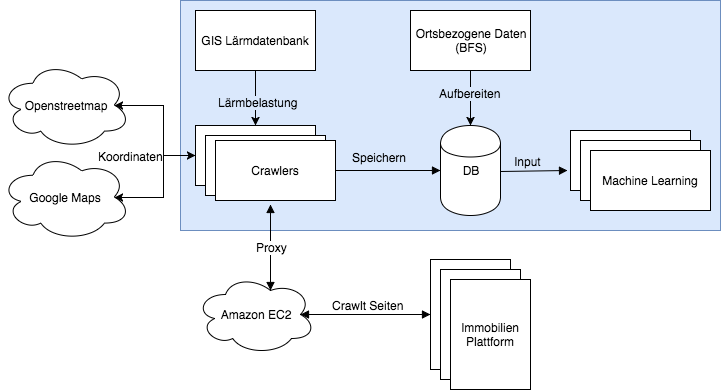
\includegraphics[width=\textwidth]{images/Architektur.png}
\caption[Systemaufbau des Projektes]{Systemaufbau des Projektes}%
\label{fig:system}
\end{figure}
Es gibt diverse Schnittstellen zu externen APIs oder Datenbanken, die wir verwenden um zusätzliche Informationen zu bekommen. Die drei wichtigsten Komponenten sind:
\begin{description}
\item[Crawler:] Sie sammeln die Immobiliendaten auf den verschiedenen Portalen. Die Crawler besitzen diverse Schnittstellen zu anderen Anbieter wie auch Datenbanken. 
\item[Datenbank:] Die Datenbank ist die zentrale Speicherstelle für unsere Inserate. Die Datenbank wurde ganz am Anfang mit ortsbezogenen Daten vom Bundesamt für Statistik befüllt. 
\item[Machine Learning:] Die Daten für das Datenset werden aus der Datenbank geladen und für die verschiedenen Algorithmen bereitgestellt.
\end{description}
In den folgenden Kapiteln wird auf diese drei Komponente genauer eingegangen.
%
\subsection{Aufbau Crawler}
Für diese Arbeit wird Scrapy als Webcrawler verwendet. Scrapy ist ein mächtiges, in Python geschriebenes, Open Source Crawler Framework.\\
Scrapy wurde ausgewählt, da es sich als Python Framework sehr gut in die Entwicklungsumgebung einfügt und es einfach anzuwenden ist \cite{scrapy}.\\
Weiter bietet Scrapy eine Item Pipeline an, um gesammelte Daten weiter zu verarbeiten. Der Vorteil der Pipeline ist, dass es erlaubt unabhängige sowie auch abhängige Schritte der Reihe nach isoliert durchzuführen. Abbildung \ref{fig:scrapy} zeigt den Aufbau der verwendeten Pipeline für das Sammeln von Immobiliendaten.\\[2ex]
\begin{figure}[h!]
\centering

\includegraphics[width=\textwidth]{images/scrapy.png}
\caption[Scrapy Pipeline]{Scrapy Pipeline}%
\label{fig:scrapy}
\end{figure}
\newline
%
\textbf{Crawlen der Webseiten}\\
Für das Crawlen der Kaufobjekte auf einer Immobilienplattform werden fokussierte Crawler verwendet. Da es zahlreiche Immobilienplattformen in der Schweiz gibt, wurden vier der grössten Plattformen ausgesucht, siehe Tabelle \ref{tab:portals}. Die Grösse definiert sich an der Anzahl Inseraten, die auf einer Seite ausgeschrieben sind. Dafür wurde die Rankingliste von Comparis genommen.\\
Um nicht als Crawler aufzufallen wurde mit Scrapoxy auf Amazon mehrere Proxy Instanzen gestartet. Diese wurden im 10-Minuten Takt terminiert und neue gestartet, um immer frische IP-Adressen zu erhalten. Da Amazon keine schweizer Server anbietet, konnten nur Portale angesteuert werden, die ausländische IP-Adressen zulassen. Comparis als grösstes Portal sperrt alle ausländischen IP-Adressen und ist so für uns nicht benutzbar.\\[2ex]
\begin{table*}[ht]
\centering
\ra{1.3}
\begin{tabular}{@{}lr@{}}
\toprule
Portal & Anzahl Inserate \\
\midrule
Homegate & 85'358\\
Immoscout & 65'543\\
Newhome & 42'804\\
Urbanhome & 27'092\\
\bottomrule
\end{tabular}
\caption{Anzahl verfügbare Inserate}
\label{tab:portals}
\end{table*}
%
Für jedes Immobilienportal erstellten wir einen eigenen Crawler. Um alle Immobilien der Schweiz zu erhalten, haben die Crawler 26 Einstiegs URLs. Jede URL deckt einen Kanton ab. Der Grund dafür ist, dass keine Immobilienplattform eine gesamtschweizerische Übersicht über ihre Immobilien anbietet. Die grösste Übersicht deckt einen ganzen Kanton ab. Punktuell mussten die URLs noch weiter verfeinert werden, da die Anzahl Resultate begrenzt waren.\\
Diese Einstiegsseiten beinhalten eine Liste aller verfügbaren Immobilien in diesem Kanton. Um an die detaillierten Informationen zu kommen, muss der Link zum Inserat extrahiert werden und in einem zweiten Schritt aufgerufen werden.
Demzufolge braucht ein Crawler fürs Portal zwei verschiedene Parser. Einer der die Übersicht und einer der die Detailseite parsed.\\[2ex]
%
Das Parsen der Seite erfolgt mit Hilfe von XPath. Die XPath Regeln wurden für alle Seiten im Voraus definiert. Bis auf die Bilder werden alle Informationen, die der Verkäufer eingeben kann, gesammelt (siehe Anhang).\\
Viele Immobilien sind nur wenige Tage online. Um später die Möglichkeit zu haben, weitere Informationen aus den Inseraten zu beschaffen, wurde zusätzlich der ganze HTML Code zum Inserat gespeichert.\\[2ex] 
%
\textbf{Zuordnung Gemeinde}\\
Vom Bundesamt für Statistik werden geobasierte Informationen der Gemeinden und Kantonen bezogen. Deshalb muss das Inserat anhand seiner Adresse einer Gemeinde zugeordnet werden. Dies geschieht in einem mehrstufigen Prozess.\\
Als erstes wird die Postleitzahl und die Ortschaft vom Inserat extrahiert. Danach wird anhand der Postleitzahl in der Datenbank den Gemeindenamen gesucht. Stimmt dieser mit dem gecrawlten Namen überein, kann die Zuordnung erfolgen.\\
Stimmt der Gemeindename nicht überein, existiert zusätzlich eine Zusatzspalte mit Alternativnamen für die Gemeinde.  Dies sind meist ältere Namen von Gemeinden die durch eine Fusion nicht mehr existieren.\\
Wird der gecrawlte Namen auch nicht in den Alternativnamen gefunden, kann keine Zuordnung durchgeführt werden.\\[2ex]
%
\textbf{Dublettencheck}\\
Es ist möglich, dass ein Inserat bei mehreren Plattformen online gestellt wird. Da es nicht optimal ist, wenn ein Inserat zweimal in unserem Datensatz vorkommt, wird versucht möglichst früh Dubletten zu erkennen und herauszufiltern. Der Dublettencheck überprüft die Übereinstimmung von Ortschaft, Objekttyp, Preis, Wohnfläche und Anzahl Zimmer. Sind diese Eigenschaften gleich, wird das Inserat ignoriert.\\[2ex]
%
\textbf{Auslesen der Tags}\\
Die Beschreibung eines Inserates, wie auch die Charakteristik, beinhaltet viele Informationen. Zum einen werden die Eckdaten nochmals in prosa formuliert. Zum Anderen wird die Innen- und Ausseneinrichtung, sowie die Umgebung beschrieben. Hier bietet sich an, diesen Text anhand von Natural Language Processing zu untersuchen. Dazu werden die wichtigsten Wörter extrahiert und als JSON-Liste abgespeichert.\\
Das NLTK-Module, das für solche Aufgaben gedacht ist, hat aber nur sehr wenige Stop-Wörter. Somit mussten wir uns eine eigene Stoppwörterliste zusammenstellen. Auch für die Übersetzung der einzelnen Ausdrücke haben wir ein eigenes Dictionary verwendet.\\[2ex]
%
\textbf{Koordinaten setzen}\\
Um die Koordinaten zu setzen, braucht es eine Strassenanschrift. Ist diese nicht vorhanden werden auch keine Koordinaten gesetzt. Das Beschaffen der Koordinaten ist ein mehrstufiger Prozess. Da von Google Maps eine Limite von 2500 Requests pro Tag existiert, wird versucht zuerst über die Openstreetmap API die Koordinaten zu beschaffen. Openstreetmap hat vergleichsweise zu Google viel weniger Einträge. Wenn bei Openstreetmap keine Koordinaten gefunden werden, wird die Google Maps API angesteuert.\\[2ex]
%
\textbf{Lärmbelastung}\\
Dieser Schritt ist der einzige in der Pipeline, der abhängig vom vorherigen Schritt ist. Denn sind keine Koordinaten vorhanden, kann auch keine Lärmbelastung berechnet werden. Die Lärmbelastung für die ganze Schweiz liegt in einem vom Bundesamt für Umwelt bereitgestellten GDAL-Format vor. Hierfür werden die Koordinaten in das Schweizer Koordinatensystem LV03 umgerechnet. Mit diesen kann in einem nächsten Schritt die Lärmbelastung berechnet werden.\\[2ex]
%
\textbf{Speichern}\\
Schlussendlich wird das gecrawlte und ergänzte Item in die Datenbank gespeichert.
%
%
\subsection{Datenbank}
Für die Datenbank wurde PostgreSQL\footnote{https://www.postgresql.org/} eingesetzt. Die Datenbank besteht aus drei Tabellen. In der Haupttabelle \textit{advertisements} sind alle Inserate der verschiedenen Immobilienportale gespeichert. In der Tabelle \textit{municipalities} sind alle ortsbezogenen Daten zu den Gemeinden und Kantonen abgelegt. Die Daten stammen vom Bundesamt für Statistik\footnote{https://www.bfs.admin.ch/bfs/de/home/statistiken/querschnittsthemen/raeumliche-analysen/raeumliche-gliederungen.assetdetail.2118475.html}. Für die Auswertung reichen die verschiedenen IDs der kategorischen Bezeichnungen. Für die Auswertung wurde stichpunktartig ein Mapping erstellt.
Die dritte Tabelle \textit{object\_types} beinhaltet alle Objekttypen, die beim Sammeln gefunden wurden. Sie wird autonom von den Crawlern befüllt.
\begin{figure}[h!]
\centering
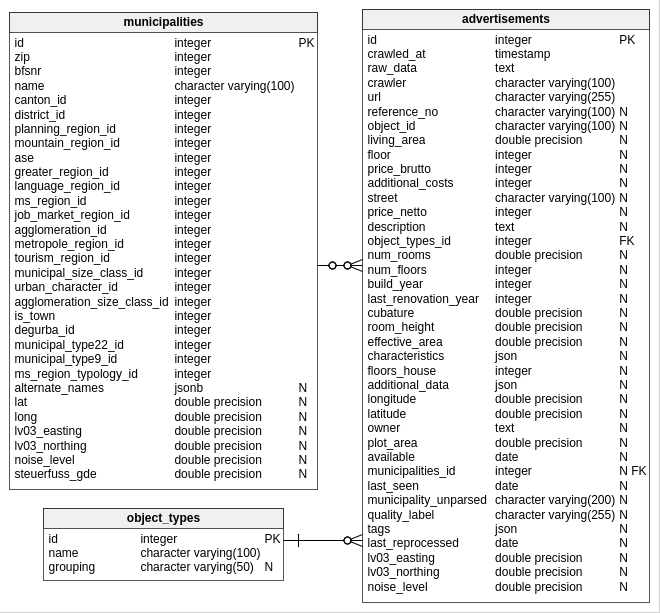
\includegraphics[width=0.9\textwidth]{images/erm.png}
\caption[Datenbankschema]{Datenbankschema}%
\label{fig:db}
\end{figure}
\newline
%
\subsection{Machine Learning}
Für Machine Learning wurde hauptsächlich mit Scikit-Learn gearbeitet \cite{scikit}. Scikit-Learn ist eine in Python geschriebene Machine Learning Library mit einer grossen Community. Punktuell wurden noch weitere ML Algorithmen verwendet, die nicht in Scikit-Learn vorhanden sind, dies wird jeweils separat erwähnt.\\[2ex]
%
Bei jedem Durchgang werden die Daten von der Datenbank geladen und denormalisiert. Da das Laden der Daten von der Datenbank Zeitintensiv ist, werden die Daten lokal zwischengespeichert.\\
Anschliessend wird ein Feature Engineering durchgeführt, bei dem diverse Daten transformiert, ergänzt oder gelöscht werden. Als weiteren Schritt, wird die Outlier Detection durchgeführt und am Ende werden diverse Machine Learning Algorithmen durchgetestet.\\[2ex]
%
\begin{figure}[h!]
\centering
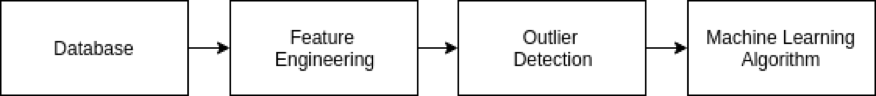
\includegraphics[width=0.9\textwidth]{images/machine_learning_pipeline.png}
\caption[Pipeline für Machine Learning]{Pipeline für Machine Learning}%
\label{fig:ml_pipeline}
\end{figure}
\newline
%
Um den ganzen Prozess einfacher zu handhaben, wurden alle Transformationen und Aktionen in möglichst kleine Funktionen verpackt, die in einer Pipeline kombiniert werden können. Somit können nach Wunsch einzelne Funktionen deaktiviert werden. Die Piepeline wird anhand einer JSON-Liste definiert. Diese Liste wird vom Programm eingelesen und der reihe nach abgearbeitet.\\[2ex]
%
Für jeden der Algorithmen wurden die diversen Parameter mit der GridSearchCV Komponente von scikit-learn durchgetestet. GridSearchCV testet für jeden Algorithmus alle Parameter mit einer Crossvalidation und gibt am Ende die Parameterwerte mit dem besten Resultat zurück. Bottleneck ist dabei die benötigte Zeit. Je nachdem wie viele Kombinationen durchgeführt werden müssen, kann das über einen Tag dauern.\\
Um nicht jedesmal eine Crossvalidation durchzuführen, werden die besten Resultate in eine Konfigurationsdatei geschrieben.\\
Der Einzige Algorithmus der nicht vom Scikit-Learn stammt, ist der XGBoost Algirthmus. Dieser wurde von Github heruntergeladen, kompiliert und das Python Paket installiert.
%
%
\subsection{Code Struktur}
Der gesamte Code mit Dokumentation wird ein einem Git Repositroy auf Github verwaltet. Git ist ein Versionsverwaltungstool. Es zeichnet auf, wer wann welche Änderungen an welchen Daten gemacht hat.\\
Die grobe Ordnerstruktur des Projektes sieht wie folgt aus:
\begin{verbatim}
immo/
  crawler
    crawler
      pipelines        # Definitionen der Pipelines
      spiders          # Definitionen der spiders
      ...
    ...
  models               # Objektdefinition
  scikit               # Machine Leraning 
    main.py            # Hauptdatei zum Starten der Pipeline
    pipeline.py        # Definitionen der verschiedenen ML-Algorithmen
    helper.py          # Anzeigen der Resultatstatistik
    data_analysis.py   # Holen und analysieren der Daten
    settings.json      # Speicherung der besten Parameter
    ...
  commands.json        # Definition der Pipeline
  ...
report                 # \LaTeX Report
daten                  # Import Daten für Datenbank
\end{verbatim}
